\section{The Chromatic Number Problem}\label{sec:chromatic}

This section investigates the various well-known methods to either estimate or find the exact chromatic number for
a graph.  Since the chromatic number problem is NP-hard, an alternative to finding an exact answer is finding lower
and upper bounds for the actual value.  If these bounds happen to match then they provide the actual chromatic
number.  Algorithms that find the exact chromatic number are of the branch and bound variety.  The two most
well-known algorithms are one proposed by Christofides~1971~\cite{christofides} with modifications by
Wang~(1974)~\cite{wang} and the so-called Zykov algorithms, with a particular implementation by Corneil and
Graham~(1973)~\cite{corneil}.

\subsection{Finding a Lower Bound}\label{sec:sub:lower}

The most popular strategy for estimating a lower bound for the chromatic number of a graph is based on the
statement of \propname~\ref{prop:clique}.  For a graph \(G\):
\[\w^*(G)\le\w(G)\le\X(G)\]
where \(\w^*(G)\) is a lower bound estimate for the clique number of \(G\).  Another less popular bound is given by
\theoremname~\ref{thm:lbalpha}~\cite{chartrand}.

\begin{theorem}
  \label{thm:lbalpha}
  Let \(G\) be a graph of order \(n\).  \(\displaystyle \X(G)\ge\frac{n}{\a(G)}\).
\end{theorem}

\begin{proof}
  Assume that \(G\) is \chromatic{k}.  This means that \(V(G)\) can be partitioned into \(k\) non-empty independent
  sets \(A_1,\ldots,A_k\), where each \(\abs{A_i}\le\a(G)\).
  \[n=\abs*{\bigcup_{1\le i\le k}A_i}=\sum_{i=1}^k\abs{A_i}\le\sum_{i=1}^k\a(G)=k\a(G)\]
  Therefore, \(\displaystyle k\ge\frac{n}{\a(G)}\).
\end{proof}

Note that both of the above lower bounds are tight when \(G\) is complete and are related by the statement of
\theoremname~\ref{thm:isclique}:
\[\w(G)=\a(\bar{G})\]

It is well-known that certain triangle-free graphs with \(\w(G)=2\) can have arbitrarily high \(\X(G)\).  Examples
are the graphs created using the so-called \emph{Mycielski} construction~\cite{west}:
\begin{enumerate}
\item Start with \(G=P_2\) \((\X(G)=2)\).
\item\label{step:myc:repeat} For the vertices in \(v\in V(G)\), create new vertices \(U=\set{u_1,\ldots,u_n}\) such
  that \(N(u_i)=N(v_i)\).  The new vertices form what is referred to as a \emph{shadow} graph.
\item Add an additional vertex \(w\) such that \(N(w)=U\) and call this new graph \(G'\), which has
  \(\X(G')=\X(G)+1\).
\item Let \(G=G'\) and go to step~\ref{step:myc:repeat}.
\end{enumerate}

The first three graphs resulting from the Mycielski construction are shown in \figurename~\ref{fig:mycielski}.

\begin{figure}[H]
  \begin{minipage}{1in}
    \centering
    \scalebox{0.75}{
      \begin{tikzpicture}[every node/.style={labeled node}, node distance=1in]
        \pathV{\(v_1\),\(v_2\)}{(0,0)}{below};
      \end{tikzpicture}
    }

    \(k=2\)
  \end{minipage}
  \begin{minipage}{2in}
    \centering
    \scalebox{0.75}{
      \begin{tikzpicture}[every node/.style={labeled node}, node distance=1in]
        \cycleV{\(v_1\),\(v_2\),\(u_1\),\(w\),\(u_2\)}{(0,0)}{0.75in}{90}{};
      \end{tikzpicture}
    }

    \(k=3\)
  \end{minipage}
  \begin{minipage}{2.75in}
    \centering
    \scalebox{0.75}{
      \begin{tikzpicture}[every node/.style={labeled node}, node distance=1in]
        \cycleV{\(v_1\),\(v_2\),\(v_3\),\(v_4\),\(v_5\)}{(0,0)}{1.25in}{90}{o};
        \cycleV{\(u_1\),\(u_2\),\(u_3\),\(u_4\),\(u_5\)}{(0,0)}{0.75in}{90}{i};
        \draw (i1) edge (o5) edge (o2);
        \draw (i2) edge (o1) edge (o3);
        \draw (i3) edge (o2) edge (o4);
        \draw (i4) edge (o3) edge (o5);
        \draw (i5) edge (o4) edge (o1);
        \node (w) at (0,0) {\(w\)};
        \draw (w) edge (i1) edge (i2) edge (i3) edge (i4) edge (i5);
      \end{tikzpicture}
    }

    \(k=4\)
  \end{minipage}
  \caption{The first three graphs from the Mycielski construction.}
  \label{fig:mycielski}
\end{figure}

The third graph in \figurename~\ref{fig:mycielski} is called the \emph{Gr\"otzsch} graph.  For another example of
triangle free graphs with arbitrarily high chromatic number, see Zhang~\cite{zhang}.  Nevertheless, for the general
case the clique number is a suitable lower bound for the chromatic number.

Unfortunately, the clique number problem for a graph \(G\) is also NP-hard, so the next best step is to use a
P-time calculation for a \(\w^*(G)\) that is as tight as possible to the actual \(\w(G)\).  Edwards and
Elphick~(1982)~\cite{edwards} investigated several such methods and concluded that the best method was a simple
calculation based on the adjacency matrix of \(G\):
\begin{enumerate}
\item Select (either lowest index or at random) a vertex \(v\in V(G)\) of maximum degree in \(G\)
  \((\deg(v)=\dmax(G))\) and let \(S=\set{v}\).
\item\label{step:edw:select} Select the vertex \(v_i\in V(G)\) such that \(v_i\notin S\) and with the minimum index
  value \(i\) that is adjacent to all of the vertices in \(S\).  If no such vertex exists then go to
  step~\ref{step:edw:done}.
\item Add \(v_i\) to \(S\) and go to step~\ref{step:edw:select}.
\item\label{step:edw:done} \(G[S]\) is a complete subgraph of \(G\) so conclude that \(\w^*(G)=\abs{S}\le\w(G)\).
\end{enumerate}

The Edwards algorithm has \(\BO(n^2)\) runtime complexity and so it is a suitable P-time algorithm.

The results of a random graph analysis of the Edwards Elphick algorithm are shown in
\figurename~\ref{fig:edwards1err}.  The graph shows edge probability versus the mean of \(\w(G)-\w^*(G)\) for
graphs of increasing order with \(1000\) trials per edge probability.  Note that the mean error increases with both
order and edge probability.

\begin{figure}[H]
  \centering
  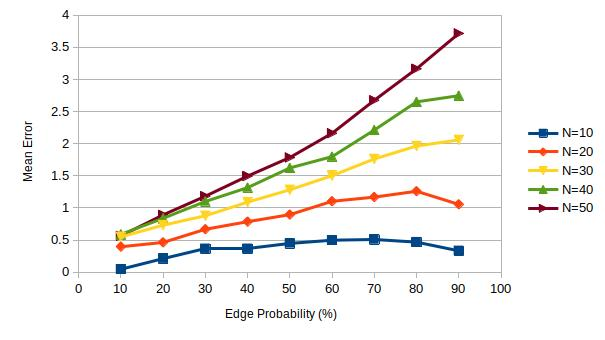
\includegraphics[width=5in]{edwards1_error}
  \caption{Edwards Elphick algorithm mean error.}
  \label{fig:edwards1err}
\end{figure}

Step~\ref{step:edw:select} of the Edwards Elphick algorithm selects the next vertex of lowest index that is
adjacent to all previously selected vertices.  An improvement would be to select a vertex with the highest degree
that is adjacent to all previously selected vertices.  This would of course increase the average runtime complexity
to the worst case of the unimproved algorithm, but it would still be P-time.  The results of this improved
algorithm are shown in \figurename~\ref{fig:edwards2err}.  Note that the improved algorithm cuts the mean error in
half.

\begin{figure}[H]
  \centering
  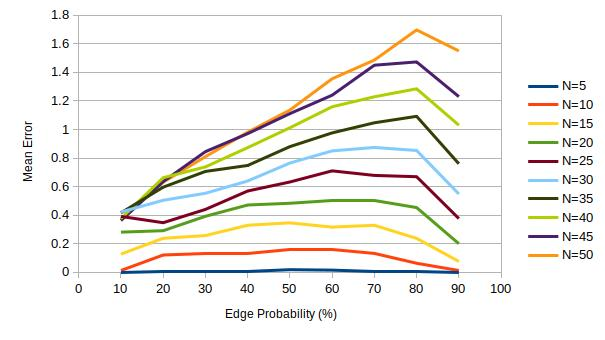
\includegraphics[width=5in]{edwards2_error}
  \caption{Improved Edwards Elphick algorithm mean error.}
  \label{fig:edwards2err}
\end{figure}

As will be shown later in this section, being able to compute the exact or a suitable estimate of the clique number
of a graph is an important bounding condition for many of the well-known branch and bound algorithms for finding
the chromatic number of a graph.  A nice summary of well-known exact clique number algorithms is given by Xiao and
Nagamouchi~(2017)~\cite{xiao}.  They claim that the known algorithms tend to converge on a runtime complexity of
\(\BO(1.2^n)\).  These algorithms tend be somewhat complex and geared towards larger \(n\).

A simpler yet efficient alternative to these exact algorithms is the Bron Kerbosch (BK)
algorithm~(1973)~\cite{bron}.  In fact, the algorithm that was incrementally developed in the previous section is
essentially the BK algorithm.  The advantage of BK is that it finds all possible maximal independent sets in a
graph, and hence can be used to find \(\a(G)=\w(\bar{G})\).  Finding all of the maximal independent sets in a graph
is a crucial part of the Christofides algorithm, which is discussed later in this section.

The heart of BK is a recursive subroutine called \emph{extend} that implements the breadth of a level in the
corresponding state tree, and recursively calls itself in order to implement the branches in the state tree.
At each node in the state tree, three vertex lists are maintained:

\begin{description}
\item[compsub] The current maximal clique accumulator.
\item[candidates] A set of vertices that can be added to \emph{compsub}.
\item[used] A set of vertices that already have been used in previous branches.
\end{description}

The initial call is seeded with an empty \emph{compsub} and all of the graph's vertices in \emph{candidates}.  Each
call to \emph{extend} performs the following steps:
\begin{enumerate}
\item\label{step:bron:check} If \emph{used} contains a vertex that is adjacent to everything in \emph{candidates}
  then any generated cliques in the current subtree will never be maximal, so return.  This implements the
  non-maximal bounding condition.
\item\label{step:bron:select} The next vertex is selected from \emph{candidates} and is added to \emph{compsub}.
  This implements the ``include vertex'' subtree.
\item\label{step:bron:recalc} New versions of \emph{candidates} and \emph{used} are created by removing vertices
  from the old lists that are not adjacent to the selected vertex.  This bounding condition prunes branches that
  might mix adjacent and nonadjacent vertices.
\item\label{step:bron:branch} A recursive call with the new \emph{candidates} and \emph{used} lists is made to
  continue the current subtree.
\item\label{step:bron:used} The selected vertex is removed from \emph{compsub} and is added to \emph{used}.  This
  implements the ``exclude vertex'' subtree.
\item\label{step:bron:leaf} If \emph{candidates} is not empty then go to step~\ref{step:bron:check}.
\item\label{step:bron:done} If \emph{used} is empty then \emph{compsub} contains the vertices for a maximal clique.
\item\label{step:bron:return} Return to the previous level in the state tree.
\end{enumerate}

A small improvement added to BK by this research is to abandon the current branch when the desire is to only find
\(\a(G)\) and the number of vertices in \emph{compsub} and \emph{candidates} are not enough to build a maximal
clique larger than all previously found maximal cliques.

Bron and Kerbosch actually proposed two versions of their algorithm that differ by how the next vertex is selected
from the \emph{candidates} list in step~\ref{step:bron:select}.  In the basic mode, the first (or any) vertex in
the list is selected.  \figurename~\ref{fig:bron1:calls} shows the average number of calls to the \emph{extend}
method versus edge probablity for \(1000\) random graphs per edge probability.

\begin{figure}[H]
  \centering
  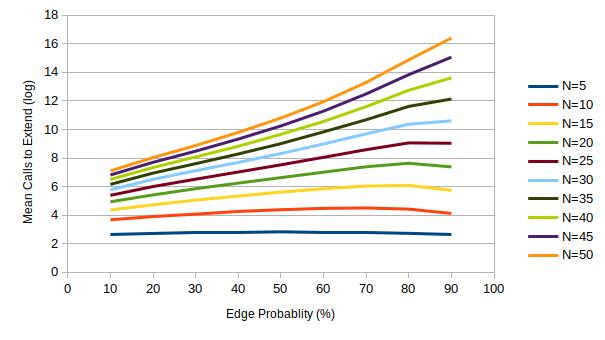
\includegraphics[width=5in]{bron1_calls}
  \caption{Basic Bron Kerbosch algorithm calls to extend versus edge probability.}
  \label{fig:bron1:calls}
\end{figure}

The number of calls increases with both graph order and edge probability.  The worst case for each order is thus
assumed to occur at \(90\%\) edge probability.  A log (base 2) plot of the maximum number of calls to the
\emph{extend} method for the \(1000\) graphs at each order is plotted in \figurename~\ref{fig:bron1:runtime}.  A
line fit is used to approximate the runtime complexity for the algorithm.  The slope of the line indicates that the
runtime complexity is about \(\BO(2^{0.3074n})\approx\BO(1.24^n)\).

\begin{figure}[H]
  \centering
  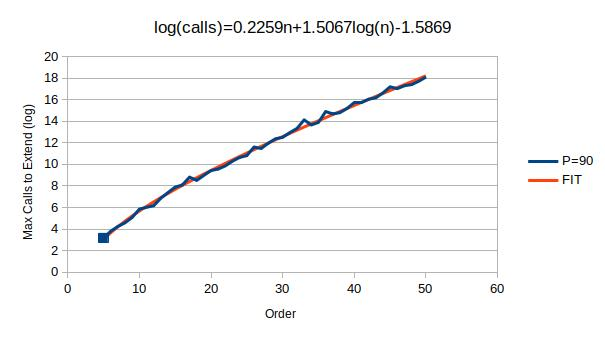
\includegraphics[width=5in]{bron1_runtime}
  \caption{Basic Bron Kerbosch algorithm runtime complexity approximation.}
  \label{fig:bron1:runtime}
\end{figure}

In smart mode, a particular vertex in the \emph{used} list with the smallest number of nonadjacencies to vertices
in the \emph{candidates} list is identified.  The next selected vertex is then a vertex that is not adjacent to the
identified vertex.  This causes the non-maximal bounding condition to occur as soon as possible.
\figurename~\ref{fig:bron2:calls} shows the average number of calls to the \emph{extend} method for the smart
version of the algorithm.

\begin{figure}[H]
  \centering
  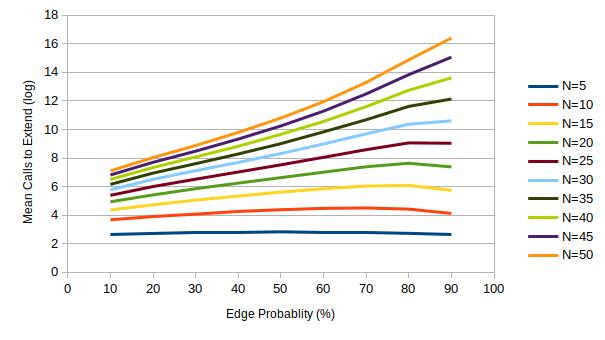
\includegraphics[width=5in]{bron1_calls}
  \caption{Smart Bron Kerbosch algorithm calls to extend versus edge probability.}
  \label{fig:bron2:calls}
\end{figure}

The runtime complexity estimate for the smart version of the algorithm is shown in
\figurename~\ref{fig:bron2:runtime}.  Note that the runtime complexity is improved to
\(\BO(2^{0.2718n})\approx\BO(1.21^n)\).

\begin{figure}[H]
  \centering
  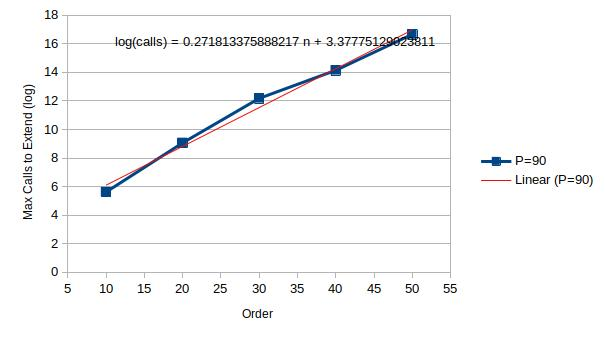
\includegraphics[width=5in]{bron2_runtime}
  \caption{Smart Bron Kerbosch algorithm runtime complexity approximation.}
  \label{fig:bron2:runtime}
\end{figure}

\subsection{Finding an Upper Bound}\label{sec:sub:upper}

The most popular technique for finding an upper bound for the chromatic number of a graph is to construct a proper
coloring for the graph using a so-called \emph{sequential} algorithm, often referred to as a \emph{greedy}
algorithm.  The algorithms are sequential because the vertices are ordered in some fashion and are then colored
according to that order.  The algorithms are greedy because a new color is selected whenever one is needed.  The
result is that too many colors may be used; however, such algorithms are P-time and the number of colors used is
suitable as an upper bound for the chromatic number since the graph is at least colorable using that many colors.

The specific steps of a greedy algorithm for a graph \(G\) of order \(n\) are as follows:
\begin{enumerate}
\item Order the vertices in some fashion: \(V=\set{v_1,\ldots,v_n}\).
\item Start with \(C=\emptyset\) and assume some coloring function: \(c:V\to C\).
\item Let \(i=1\).
\item\label{step:greedy:check} Let \(k=\abs{C}\).
\item If \(i=n\) then done and \(k\) is an upper bound for the chromatic number.
\item Determine all of the already colored vertices that are adjacent to \(v_i\):
  \[S=\setb{v_j\in V}{j<i\ \text{and}\ v_iv_j\in E(G)}\]
\item Determine all of the colors used by the vertices in \(S\): \(c[S]\).
\item If \(c[S]=C\) then an additional color is needed for \(v_i\), so add \(c_{k+1}\) to \(C\), let
  \(c_j=c_{k+1}\), and go to step~\ref{step:greedy:color}.
\item Otherwise, an existing color can be reused for \(v_i\) so select \(c_j\) from \(C-c[S]\) with the smallest
  \(j\).
\item\label{step:greedy:color} Color \(v_i\) with \(c_j\) by extending \(c\): \(c(v_i)=c_j\).
\item Let \(i=i+1\).
\item Go to step~\ref{step:greedy:check}.
\end{enumerate}

Indeed, the two most popular theorems used to quickly estimate the chromatic number upper bound of a graph follow
from the worst case result from this algorithm.  The first is based on a random ordering of the
vertices~\cite{chartrand}.

\begin{theorem}
  \label{thm:upper}
  Let \(G\) be a graph.  \(\X(G)\le1+\dmax(G)\)
\end{theorem}

The second, from Welsh and Powell (1967), is based on ordering by non-increasing vertex degree~\cite{welsh}.

\begin{theorem}
  \label{thm:welsh}
  Let \(G\) be a graph:
  \[\X(G)\le\max_i\min\left\{1+\deg(v_i),i\right\}\]
\end{theorem}

Matula, et al (1967)~\cite{matula} performed a study on the various well-known chromatic number upper bound
algorithms and concluded that ordering the vertices by non-increasing degree order, as in the Welsh Powell bound,
worked best.  Matula referred to this algorithm as the \emph{last-first} algorithm.  In fact, Matula offered an
improvement to this algorithm known as \emph{color interchange}.

Color interchange is based on the situation summarized by the example in \figurename~\ref{fig:interchange}.  When it
is time to color \(v_4\), the normal greedy algorithm is forced to select a new color.  However, vertices \(v_1\)
and \(v_3\) can swap colors and thus \(v_4\) can use an existing color.

\begin{figure}[H]
  \begin{minipage}{2.5in}
    \centering
    \begin{tikzpicture}[every node/.style={labeled node}]
      \colorlet{c1}{green!25!white}
      \colorlet{c2}{red!25!white}
      \node (4) at (0,0) {\(v_4\)};
      \node [fill=c1] (1) at (2,1) {\(v_1\)};
      \node [fill=c2] (2) at (2,-1) {\(v_2\)};
      \node [fill=c2] (3) at (4,1) {\(v_3\)};
      \draw (4) edge (1) edge (2);
      \draw (1) edge (3);
    \end{tikzpicture}

    Before Swap
  \end{minipage}
  \begin{minipage}{2.5in}
    \centering
    \begin{tikzpicture}[every node/.style={labeled node}]
      \colorlet{c1}{green!25!white}
      \colorlet{c2}{red!25!white}
      \node (4) at (0,0) {\(v_4\)};
      \node [fill=c2] (1) at (2,1) {\(v_1\)};
      \node [fill=c2] (2) at (2,-1) {\(v_2\)};
      \node [fill=c1] (3) at (4,1) {\(v_3\)};
      \draw (4) edge (1) edge (2);
      \draw (1) edge (3);
    \end{tikzpicture}

    After Swap
  \end{minipage}
  \caption{An example that allows color interchange.}
  \label{fig:interchange}
\end{figure}

The specific steps for color interchange when attempting to color vertex \(v_i\) are as follows:
\begin{enumerate}
\item Determine all of the colors that are used for already colored vertices that are adjacent to \(v_i\).
\item Select those colors that occur only once in the neighborhood of \(v_i\).
\item Select all vertices that are already colored with the used-once colors.
\item Construct a subgraph using the selected vertices.
\item\label{step:color:part} Partition the subgraph into components.
\item Find a component that includes one vertex and excludes one vertex that is adjacent to \(v_i\) in the original
  graph.  If no such component is found then interchange is not possible and a new color must be used for \(v_i\).
\item Let \(c_1\) be the color of the included vertex and let \(c_2\) be the color of the excluded vertex.
\item Interchange colors \(c_1\) and \(c_2\) for all such colored vertices in the selected component.
\item Color \(c_1\) is now available for \(v_i\).
\end{enumerate}

The results of a random graph analysis of the last-first greedy algorithm with color interchange are shown in
\figurename~\ref{fig:greedyerr}.  The previously mentioned Hopcroft algorithm~\cite{hopcroft} was used to partition
the subgraph in step~\ref{step:color:part}.  The graph shows edge probability versus the mean of the difference
between the greedy value and the actual chromatic number for graphs of increasing order with \(10\) trials per edge
probability.  Note that the algorithm tends to do better at lower and higher edge densities.

\begin{figure}[H]
  \centering
  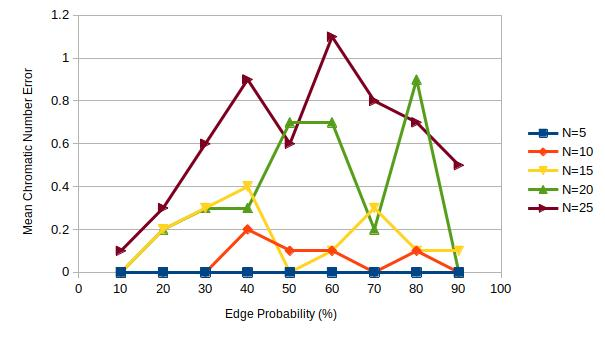
\includegraphics[width=5in]{greedy_error}
  \caption{Last first greedy algorithm with interchange error versus edge probability.}
  \label{fig:greedyerr}
\end{figure}

Although still P-time, the interchange portion of the algorithm is stepwise expensive.  A random graph analysis was
performed on \(1000\) graphs per various edge probabilities and graph order comparing upper bound values from
greedy coloring with and without color interchange.  The results for \(n=50\) are typical and are shown in
\tablename~\ref{tab:greedy}.  The mean, min, and max for greedy coloring without interchange minus greedy coloring
with interchange are shown.  The data suggests that color interchange might not be very much of a benefit.

\begin{table}[H]
  \centering
  \caption{Effectiveness of Color Interchange}
  \label{tab:greedy}
  \begin{tabular}{|c|c|c|c|}
    \hline
    edge prob (\%) & mean & min & max \\
    \hline
    10 & 0.04 & -1 & 1 \\
    \hline
    20 & 0.023 & -1 & 2 \\
    \hline
    30 & 0.027 & -2 & 2 \\
    \hline
    40 & 0.016 & -2 & 2 \\
    \hline
    50 & 0.008 & -2 & 2 \\
    \hline
    60 & -0.005 & -3 & 2 \\
    \hline
    70 & -0.001 & -2 & 2 \\
    \hline
    80 & 0.001 & 0 & 1 \\
    \hline
    90 & 0 & 0 & 0 \\
    \hline
  \end{tabular}
\end{table}

\subsection{The Christofides Algorithm}\label{sec:sub:christofides}

The first exhaustive algorithm that will be examined was proposed by Cypriot mathematician Nicos
Christofides~(1971)~\cite{christofides}.  The Christofides algorithm is a breadth-first algorithm that assembles
maximal independent sets from a graph until the first combination that uses all of the vertices is found.  Thus,
the Bron Kerbosch algorithm is a vital part of the Christofides algorithm.

The Christofides algorithm starts by decomposing a graph \(G\) into all of its maximal independent sets.  This
constitutes the first level of the state tree.  Then, for each maximal independent set with vertices \(S\), the
subgraph \(G-S\) is constructed and all of its maximal independent sets are found.  Each of these sets is combined
with the previous maximal independent sets to form the next layer of the state tree.  This process continues until
the first time that all of the vertices in \(G\) are used.  The number of maximal independent sets used to form the
final combination is the chromatic number.

The Christofides does have bounding conditions.  If the vertices in any new combination of maximal independent sets
is a subset of a previous combination then the subtree for the latter is pruned.  If the former is a subset of the
latter then the former subtree is pruned by replacing its state with the state of the latter.

For example, consider the graph in \figurename~\ref{fig:cfexample}.

\begin{figure}[H]
  \centering
  \begin{tikzpicture}
    \cycleNnodes{5}{(0,0)}{0.75in}{90}{c};
    \begin{scope}[every node/.style={labeled node}]
      \node (1) at (c1) {\(1\)};
      \node (2) at (c2) {\(2\)};
      \node (3) at (c3) {\(3\)};
      \node (4) at (c4) {\(4\)};
      \node (5) at (c5) {\(5\)};
    \end{scope}
    \draw (1) edge (2) edge (3) edge (4) edge (5);
    \draw (2) edge (3);
    \draw (3) edge (4);
    \draw (4) edge (5);
  \end{tikzpicture}
  \caption{A Christofides algorithm example.}
  \label{fig:cfexample}
\end{figure}

The Bron Kerbosch algorithm is used to decompose \figurename~\ref{fig:cfexample} into the maximal independent sets
\(\set{1}\), \(\set{2,4}\), \(\set{2,5}\), and \(\set{3,5}\).  This first level is shown in
\figurename~\ref{fig:cflevel1}, along with the resulting subgraphs.

\begin{figure}[H]
  \begin{minipage}{1.5in}
    \centering
    \((1)\)

    \bigskip

    \begin{tikzpicture}
      \cycleNnodes{5}{(0,0)}{0.5in}{90}{c};
      \begin{scope}[every node/.style={labeled node}]
        \node (2) at (c2) {\(2\)};
        \node (3) at (c3) {\(3\)};
        \node (4) at (c4) {\(4\)};
        \node (5) at (c5) {\(5\)};
      \end{scope}
      \draw (2) edge (3);
      \draw (3) edge (4);
      \draw (4) edge (5);
    \end{tikzpicture}
  \end{minipage}
  \begin{minipage}{1.25in}
    \centering
    \((2,4)\)

    \bigskip

    \begin{tikzpicture}
      \cycleNnodes{5}{(0,0)}{0.5in}{90}{c};
      \begin{scope}[every node/.style={labeled node}]
        \node (1) at (c1) {\(1\)};
        \node (3) at (c3) {\(3\)};
        \node (5) at (c5) {\(5\)};
      \end{scope}
      \draw (1) edge (3) edge (5);
    \end{tikzpicture}
  \end{minipage}
  \begin{minipage}{1.25in}
    \centering
    \((2,5)\)

    \bigskip

    \begin{tikzpicture}
      \cycleNnodes{5}{(0,0)}{0.5in}{90}{c};
      \begin{scope}[every node/.style={labeled node}]
        \node (1) at (c1) {\(1\)};
        \node (3) at (c3) {\(3\)};
        \node (4) at (c4) {\(4\)};
      \end{scope}
      \draw (1) edge (3) edge (4);
      \draw (3) edge (4);
    \end{tikzpicture}
  \end{minipage}
  \begin{minipage}{1.25in}
    \centering
    \((3,5)\)

    \bigskip

    \begin{tikzpicture}
      \cycleNnodes{5}{(0,0)}{0.5in}{90}{c};
      \begin{scope}[every node/.style={labeled node}]
        \node (1) at (c1) {\(1\)};
        \node (2) at (c2) {\(2\)};
        \node (4) at (c4) {\(4\)};
      \end{scope}
      \draw (1) edge (2) edge (4);
    \end{tikzpicture}
  \end{minipage}
  \caption{Level 1 of a Christofides algorithm example.}
  \label{fig:cflevel1}
\end{figure}

The next level starts with the leftmost subgraph in \figurename~\ref{fig:cflevel1}.  It has the maximal independent
sets \(\set{2,4}\) and \(\set{3,5}\).  These are combined with the parent state to form the next states
\(\set{\set{1},\set{2,4}}\) and \(\set{\set{1},\set{3,5}}\).  Likewise, the second graph in
\figurename~\ref{fig:cflevel1} contains maximal independent sets \(\set{1}\) and \(\set{3,5}\).  This yields the
next states \(\set{\set{2,4},\set{1}}\) and \(\set{\set{2,4},\set{3,5}}\); however, the vertices in
\(\set{\set{2,4},\set{1}}\) are a subset of the previous state \(\set{\set{1},\set{2,4}}\) and so the new subtree
is pruned.  This process continues for the third and fourth subgraph in \figurename~\ref{fig:cflevel1}.  The second
level results are as follows:

\begin{tabular}{ccccccccc}
  \((1|24)\) & \((1|35)\) & \(\cancel{(24|1)}\) & \((24|35)\) & \((25|1)\) & \(\cancel{(25|3)}\) &
  \(\cancel{(25|4)}\) & \(\cancel{(35|1)}\) & \(\cancel{(35|24)}\)
\end{tabular}

Next, the first state in the second level contains a single maximal independent set \(\set{3,5}\), which when
combined with the parent state uses all of the vertices.  The final coloring is thus \((1|24|35)\) and the graph is
\chromatic{3} as shown in \figurename~\ref{fig:cfresults}.

\begin{figure}[H]
  \centering
  \begin{tikzpicture}
    \colorlet{clr1}{red!25!white}
    \colorlet{clr2}{green!25!white}
    \colorlet{clr3}{blue!25!white}
    \cycleNnodes{5}{(0,0)}{0.75in}{90}{c};
    \begin{scope}[every node/.style={labeled node}]
      \node [fill=clr1] (1) at (c1) {\(1\)};
      \node [fill=clr2] (2) at (c2) {\(2\)};
      \node [fill=clr3] (3) at (c3) {\(3\)};
      \node [fill=clr2] (4) at (c4) {\(4\)};
      \node [fill=clr3] (5) at (c5) {\(5\)};
    \end{scope}
    \draw (1) edge (2) edge (3) edge (4) edge (5);
    \draw (2) edge (3);
    \draw (3) edge (4);
    \draw (4) edge (5);
  \end{tikzpicture}
  \caption{Christofides algorithm example results.}
  \label{fig:cfresults}
\end{figure}

The results of a random graph analysis of the Christofides algorithm are shown in \figurename~\ref{fig:cfstates}.
The graph shows edge probability versus the mean of the number of states for graphs of increasing order with \(10\)
trials per edge probability.  The limited number of trials is due to the required time duration at higher orders.

\begin{figure}[H]
  \centering
  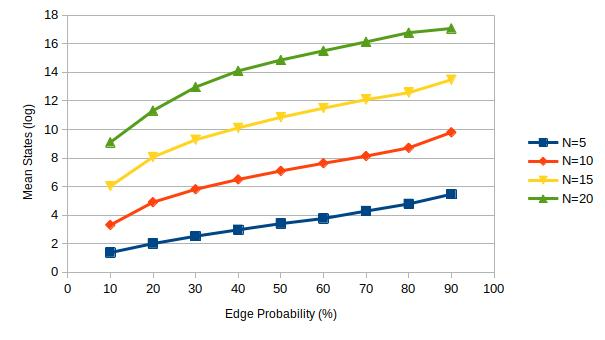
\includegraphics[width=5in]{christofides_states}
  \caption{Chistofides algorithm mean number of states.}
  \label{fig:cfstates}
\end{figure}

The number of states increases with both graph order and edge probability.  The worst case for each order is thus
assumed to occur at \(90\%\) edge probability.  A log (base 2) plot of the maximum number of states for the \(10\)
graphs at each order is plotted in \figurename~\ref{fig:cfruntime}.  A line fit is used to approximate the runtime
complexity for the algorithm.  The slope of the line indicates that the runtime complexity is about
\(\BO(2^{0.8393n})\approx\BO(1.79^n)\).

\begin{figure}[H]
  \centering
  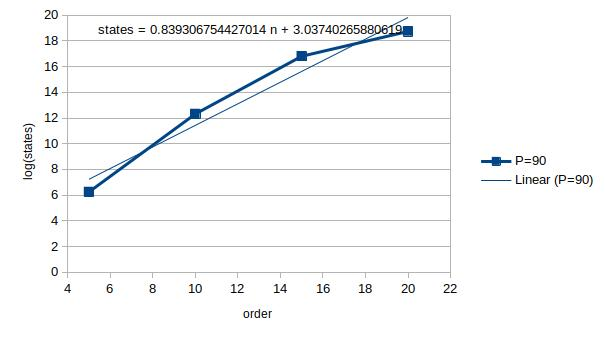
\includegraphics[width=5in]{christofides_runtime}
  \caption{Christofides algorithm runtime complexity approximation.}
  \label{fig:cfruntime}
\end{figure}

\subsection{Zykov Algorithms}\label{sec:sub:zykov}

An exhaustive, exponential-time algorithm for determining the chromatic number of a graph is derived from a
nondeterministic Turing machine technique attributed to Ukranian graph theorist Alexandre A. Zykov (1922--2013)
\cite{obit}.

\begin{figure}[h]
  \label{fig:zykov}
  \begin{center}
    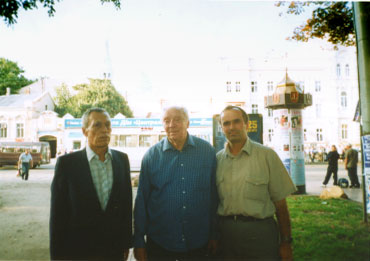
\includegraphics{zykov}
  \end{center}
  \caption{V.G Vizing (L), A.A. Zykov (C), and V.I. Voloshin (R) in Odessa (2001) \cite{voloshin}}
\end{figure}

\subsubsection{The Chromatic Polynomial}

In his 1949 paper (translated by the AMS in 1952) \cite{zykov}, Zykov addresses the question: given a graph \(G\) and
a number \(k\in\N\), how many ways are there to properly color \(G\) using at most \(k\) colors?  In fact, he is not
particularly concerned about the chromatic number, which he calls the \emph{rank}, of a graph.  To solve this problem,
Zykov notes that in any proper coloring of a graph:
\begin{enumerate}
\item Nonadjacent vertices have either the same color or different colors.
\item Adjacent vertices always have different colors.
\end{enumerate}
If nonadjacent vertices have the same color then they can be contracted and the resulting graph retains the same
\coloring{k} as the original graph.  This is demonstrated in Figure \ref{fig:zvcon}.

\begin{figure}[h]
  \label{fig:zvcon}
  \begin{center}
    \begin{minipage}{2in}
      \begin{center}
        \begin{tikzpicture}[every node/.style={labeled node}]
          \colorlet{c1}{green!25!white}
          \colorlet{c2}{blue!25!white}
          \colorlet{c3}{red!25!white}
          \node (d) [fill=c2] at (0,0) {\(d\)};
          \node (c) [fill=c3,right=of d] {\(c\)};
          \node (b) [fill=c2,above=of c] {\(b\)};
          \node (a) [fill=c1,above=of d] {\(a\)};
          \draw (a) -- (b);
          \draw (a) -- (c) -- (d) -- (a);
        \end{tikzpicture}

        \bigskip

        \(G\)
      \end{center}
    \end{minipage}
    \begin{minipage}{2in}
      \begin{center}
        \begin{tikzpicture}[every node/.style={labeled node}]
          \colorlet{c1}{green!25!white}
          \colorlet{c2}{blue!25!white}
          \colorlet{c3}{red!25!white}
          \node (bd) [fill=c2] at (0,0) {\(bd\)};
          \node (c) [fill=c3,right=of bd] {\(c\)};
          \node (a) [fill=c1,above=of bd] {\(a\)};
          \draw (a) -- (c) -- (bd) -- (a);
        \end{tikzpicture}

        \bigskip

        \(G\cdot bd\)
      \end{center}
    \end{minipage}
  \end{center}
  \caption{Same Colors with Vertex Contraction}
\end{figure}

If nonadjacent vertices have different colors then they can be joined by an edge and the resulting graph retains
the same \coloring{k} as the original graph.  This is demonstrated in Figure \ref{fig:zeadd}.

\begin{figure}[h]
  \label{fig:zeadd}
  \begin{center}
    \begin{minipage}{2in}
      \begin{center}
        \begin{tikzpicture}[every node/.style={labeled node}]
          \colorlet{c1}{green!25!white}
          \colorlet{c2}{blue!25!white}
          \colorlet{c3}{red!25!white}
          \node (d) [fill=c2] at (0,0) {\(d\)};
          \node (c) [fill=c3,right=of d] {\(c\)};
          \node (b) [fill=c2,above=of c] {\(b\)};
          \node (a) [fill=c1,above=of d] {\(a\)};
          \draw (a) -- (b);
          \draw (a) -- (c) -- (d) -- (a);
        \end{tikzpicture}

        \bigskip

        \(G\)
      \end{center}
    \end{minipage}
    \begin{minipage}{2in}
      \begin{center}
        \begin{tikzpicture}[every node/.style={labeled node}]
          \colorlet{c1}{green!25!white}
          \colorlet{c2}{blue!25!white}
          \colorlet{c3}{red!25!white}
          \node (d) [fill=c2] at (0,0) {\(d\)};
          \node (c) [fill=c3,right=of d] {\(c\)};
          \node (b) [fill=c2,above=of c] {\(b\)};
          \node (a) [fill=c1,above=of d] {\(a\)};
          \draw (a) -- (b) -- (c);
          \draw (a) -- (c) -- (d) -- (a);
        \end{tikzpicture}

        \bigskip

        \(G+bc\)
      \end{center}
    \end{minipage}
  \end{center}
  \caption{Different Colors with Edge Addition}
\end{figure}

By applying these steps recursively, all of the possible distributions of the nonadjacent nodes to independent sets
are generated.  The termination condition for each recursive path is a complete graph of some varying order \(k\).
Each node in the complete graph represents an independent set of nonadjacent nodes in the original graph that have
been combined via vertex contraction.  Thus, each complete graph of order \(k\) represents a possible \coloring{k}
of the original graph.  The complete graphs of smallest order represent chromatic colorings and their order is the
chromatic number of the original graph.

Zykov uses a graph equation syntax to record the recursive processing of a graph, where each line in the equation
represents the next recursive layer.  Isomorphic graphs are combined with a frequency multiplier at each layer.
This is demonstrated in Figure \ref{fig:greqn}.

\begin{figure}[h]
  \label{fig:greqn}
  \begin{align*}
    \begin{minipage}{0.75in}
      \begin{center}
        \begin{tikzpicture}[every node/.style={unlabeled node}]
          \node (a1) at (0,0) {};
          \node (a2) [right=of a1] {};
          \node (a3) [above=of a2] {};
          \node (a4) [above=of a1] {};
          \draw (a3) -- (a4) -- (a1) -- (a2) -- (a4);
        \end{tikzpicture}
      \end{center}
    \end{minipage} &=
    \begin{minipage}{0.75in}
      \begin{center} 
        \begin{tikzpicture}[every node/.style={unlabeled node}]
          \node (b1) at (0,0) {};
          \node (b2) [above=of b1] {};
          \node (b3) [right=of b1] {};
          \draw (b1) -- (b2) -- (b3) -- (b1);
        \end{tikzpicture}
      \end{center}
    \end{minipage} +
    \begin{minipage}{0.75in}
      \begin{center}
        \begin{tikzpicture}[every node/.style={unlabeled node}]
          \node (c1) at (0,0) {};
          \node (c2) [right=of a1] {};
          \node (c3) [above=of a2] {};
          \node (c4) [above=of a1] {};
          \draw (c2) -- (c3) -- (c4) -- (c1) -- (c2) -- (c4);
        \end{tikzpicture}
      \end{center}
    \end{minipage} \\
    &= \begin{minipage}{0.75in}
      \begin{center} 
        \begin{tikzpicture}[every node/.style={unlabeled node}]
          \node (b1) at (0,0) {};
          \node (b2) [above=of b1] {};
          \node (b3) [right=of b1] {};
          \draw (b1) -- (b2) -- (b3) -- (b1);
        \end{tikzpicture}
      \end{center}
    \end{minipage} +
    \begin{minipage}{0.75in}
      \begin{center} 
        \begin{tikzpicture}[every node/.style={unlabeled node}]
          \node (b1) at (0,0) {};
          \node (b2) [above=of b1] {};
          \node (b3) [right=of b1] {};
          \draw (b1) -- (b2) -- (b3) -- (b1);
        \end{tikzpicture}
      \end{center}
    \end{minipage} +
    \begin{minipage}{0.75in}
      \begin{center}
        \begin{tikzpicture}[every node/.style={unlabeled node}]
          \node (c1) at (0,0) {};
          \node (c2) [right=of a1] {};
          \node (c3) [above=of a2] {};
          \node (c4) [above=of a1] {};
          \draw (c2) -- (c3) -- (c4) -- (c1) -- (c2) -- (c4);
          \draw (c1) -- (c3);
        \end{tikzpicture}
      \end{center}
    \end{minipage} \\
    &= 2
    \begin{minipage}{0.75in}
      \begin{center} 
        \begin{tikzpicture}[every node/.style={unlabeled node}]
          \node (b1) at (0,0) {};
          \node (b2) [above=of b1] {};
          \node (b3) [right=of b1] {};
          \draw (b1) -- (b2) -- (b3) -- (b1);
        \end{tikzpicture}
      \end{center}
    \end{minipage} +
    \begin{minipage}{0.75in}
      \begin{center}
        \begin{tikzpicture}[every node/.style={unlabeled node}]
          \node (c1) at (0,0) {};
          \node (c2) [right=of a1] {};
          \node (c3) [above=of a2] {};
          \node (c4) [above=of a1] {};
          \draw (c2) -- (c3) -- (c4) -- (c1) -- (c2) -- (c4);
          \draw (c1) -- (c3);
        \end{tikzpicture}
      \end{center}
    \end{minipage} \\
    &= 2K_3+K_4
  \end{align*}
  \caption{Zykov Graph Equation}
\end{figure}

Determining whether two graphs are isomorphic is hard, so combining isomorphic graphs in all but the very simple
cases should be skipped; the complete graphs resulting from the further processing of two isomorphic graphs will
eventually be combined anyway by the end.

Zykov was trying to determine the number of \coloring{k}s of a graph without color indifference: each permutation
of colors for a particular distribution is considered unique.  Thus, Zykov multiplied each complete graph
coefficient in the final line of a graph equation by the number of permutations from selecting the order \(n\) of
the particular complete graph from \(k\) colors:
\[k^{(n)}=k(k-1)(k-2)\cdots(k-n+1)\]
Thus, the total number of unique colorings from the example shown in Figure \ref{fig:greqn} using \(k\) colors
would be:
\[M(G,k)=2k^{(3)}+k^{(4)}\]
This is known as the factorial form of the \emph{chromatic polynomial} for the graph.  The corresponding
\emph{expanded form} is:
\[M(G,k)=k^4-4k^3+5k^2-2k\]
Read (1968) \cite{read} expands on the construction of the factorial form of the chromatic polynomial for a graph
and proves several theorems regarding the expanded form.  Some examples are:
\begin{enumerate}
\item \(M(G,k)=M(G\cdot uv)+M(G+uv)\), where \(u\) and \(v\) are any two nonadjacent vertices in the current
  recursive step.
\item The degree of M(G,k) is the order of \(G\).
\item The highest order coefficient is \(1\).
\item There is no constant term.
\item The terms alternate in sign.
\end{enumerate}
In fact, Read shows that the expanded form is actually an inclusion-exclusion equation resulting from starting with
all possible proper and improper colorings \(k^n\) and then subtracting the improper colorings.

\subsubsection{An Exhaustive Algorithm}

Corneil and Graham extend Zykov's work with the following theorem \cite{corneil}:

\begin{theorem}[Corneil and Graham, 1973]
  \label{thm:corneil}
  Let \(G\) be a graph and let \(u\) and \(v\) be two nonadjacent vertices in \(G\):
  \[\X(G)=\min\set{\X(G\cdot uv),\X(G+uv)}\]
\end{theorem}

Zykov's method combined with Theorem \ref{thm:corneil} can be used to construct an exhaustive algorithm for finding
the chromatic number and a chromatic coloring for a graph \(G\).  We define \(S\) to be a first-in-first out (FIFO)
stack of graphs and \(X\) to be the last found complete graph of the smallest order.  Each vertex in \(X\)
represents a set of contracted vertices.
\begin{enumerate}
\item Construct a graph \(G'\) that is isomorphic to \(G\) and where each vertex in \(G'\) is a list of contracted
  vertices initialized to a one element list containing the corresponding vertex in \(G\).
\item Push \(G'\) onto \(S\).
\item \label{step:zempty} If \(S\) is empty then return \(n(X)\) and \(X\).
\item \label{step:zcheck} If the graph on the top of \(S\) is complete:
  \begin{enumerate}
  \item Pop the graph off of the top of \(S\) and save it as \(H\).
  \item If \(X\) is not set or \(n(H)<n(X)\) then let \(X=H\).  Otherwise, discard \(H\).
  \item Go to step \ref{step:zempty}.
  \end{enumerate}
\item The graph on the top of \(S\) is not complete.  Pop the graph off of \(S\) and save it as \(H\).
\item Pick any two nonadjacent vertices \(u\) and \(v\) in \(H\).
\item Push \(H+uv\) onto \(S\).
\item Construct \(H'=H\cdot uv\), where the contracted vertex list for the new contracted vertex is a concatenation
  of the lists for \(u\) and \(v\).
\item Push \(H'\) onto \(S\).
\item Go to step \ref{step:zcheck}.
\end{enumerate}

The steps of this algorithm can be tracked via a so-called \emph{Zykov tree} \cite{corneil}.  The Zykov tree for
the example in Figure \ref{fig:greqn} is shown in Figure \ref{fig:ztree}.  Note that the exhaustive algorithm
corresponds to a depth-first walk of the tree.

\begin{figure}[h]
  \label{fig:ztree}
  \begin{center}
    \begin{tikzpicture}
      \node (a) [draw,circle] at (0,0) {
        \begin{tikzpicture}[every node/.style={unlabeled node}]
          \node (a1) at (0,0) {};
          \node (a2) [right=of a1] {};
          \node (a3) [above=of a2] {};
          \node (a4) [above=of a1] {};
          \draw (a3) -- (a4) -- (a1) -- (a2) -- (a4);
        \end{tikzpicture}
      };
      \node (b) [draw,circle,below left=of a] {
        \begin{tikzpicture}[every node/.style={unlabeled node}]
          \node (b1) at (0,0) {};
          \node (b2) [above=of b1] {};
          \node (b3) [right=of b1] {};
          \draw (b1) -- (b2) -- (b3) -- (b1);
        \end{tikzpicture}
      };
      \node (c) [draw,circle,below right=of a] {
        \begin{tikzpicture}[every node/.style={unlabeled node}]
          \node (c1) at (0,0) {};
          \node (c2) [right=of a1] {};
          \node (c3) [above=of a2] {};
          \node (c4) [above=of a1] {};
          \draw (c2) -- (c3) -- (c4) -- (c1) -- (c2) -- (c4);
        \end{tikzpicture}
      };
      \node (d) [draw,circle,below left=of c] {
        \begin{tikzpicture}[every node/.style={unlabeled node}]
          \node (d1) at (0,0) {};
          \node (d2) [above=of d1] {};
          \node (d3) [right=of d1] {};
          \draw (d1) -- (d2) -- (d3) -- (d1);
        \end{tikzpicture}
      };
      \node (e) [draw,circle,below right=of c] {
        \begin{tikzpicture}[every node/.style={unlabeled node}]
          \node (c1) at (0,0) {};
          \node (c2) [right=of a1] {};
          \node (c3) [above=of a2] {};
          \node (c4) [above=of a1] {};
          \draw (c2) -- (c3) -- (c4) -- (c1) -- (c2) -- (c4);
          \draw (c1) -- (c3);
        \end{tikzpicture}
      };
      \draw (a) edge (b) edge (c);
      \draw (c) edge (d) edge (e);
    \end{tikzpicture}
  \end{center}
  \caption{A Zykov Tree}
\end{figure}

\subsubsection{Branch and Bound Strategies}

Using a Zykov tree suggests that the exhaustive algorithm is a candidate for a branch-and-bound solution, where the
branching is accomplished via vertex contraction and edge addition and the bounding is some method to prematurely
terminate a branch.  Corneil and Graham suggest such a bounding technique through the determination of so-called
\(\a\)-clusters; however, the algorithm for finding such clusters has \(\BO(n^3)\) runtime complexity.
